\section{User}

På WePlanner kan man registrere sig og logge ind som bruger. User Stories for en bruger, og arkitekturen som bliver bygget på baggrund af disse userstories vil blive gennemgået i dette afsnit. Der vil blive gennemgået database arkitektur i Data View, samt den logiske arkitektur under Logical View.
\newline 
User Stories for User kan ses herunder:

\begin{itemize}
    \item Opret Bruger (I)
    \item Log Ind (I)
    \item Ændring af navn, password og e-mail (I)
    \item Indstil profilbillede og personligt tema
    \item Tilknyt Facebook Konto*
\end{itemize}

* Ikke implementeret \newline
(I) Identity framework

I .NET Frameworks MVC projekt, kan man vælge at bygge med Identity Framework, hvilket giver projektet registrering og login funktionalitet. Derfor blev dette valgt, eftersom det udfylder de 3 første userstories ovenfor. Disse userstories vil derfor ikke blive beskrevet i arkitekturafsnittet.

User Storien "Opret gruppe", bliver beskrevet i Groups afsnittet, og vil derfor ikke blive beskrevet her.
Derfor vil der kun blive beskrevet arkitekturen for usermodellen, samt indstilling af profilbillede.

\subsection{Data View}
Som nævnt tidligere, så er meget af usermodellen givet på forhånd i Identity Framework. Derfor har projektgruppen altså ikke haft behov for at tilføje password, username, og email i usermodellen. Der er dog nogle attributer som skulle tilføjes, som kan ses på ER modellen på figur \ref{fig:ER_Model_User}:

\begin{figure}[H]
    \centering
    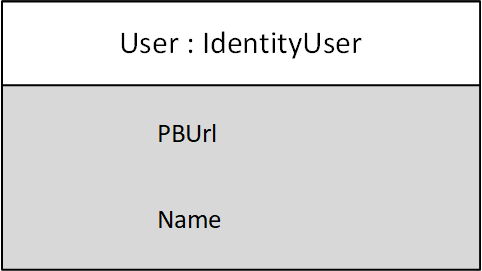
\includegraphics[width=0.45\linewidth]{09_Arkitektur/User/Images/User_DatabaseModel.png}
    \caption{User ER Model}
    \label{fig:ER_Model_User}
\end{figure}

Som der kan ses er der blevet tilføjet et Navn, som er en brugers nickname. Derudover er der sat en string ind til PBUrl. Ud over dette er der blevet lavet 4 relations til entiteterne Groups, WallPosts, GroupsAdministrators samt OwnerGroups.

\mini{Tjek om WallPosts skal fjernes}

\subsection{Logical View}

I logical view for user, er det kun user storien "Indstil profilbillede og personligt tema", som skal implementeres. På baggrund af det meget begrænsede funktionalitet som skal implementeres for user, laves der et kortfattet klassediagram, som kan ses i \ref{fig:UserController_Class}

\begin{figure}[H]
    \centering
    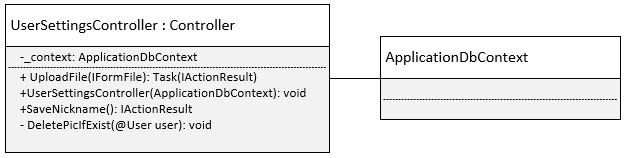
\includegraphics[width=0.9\linewidth]{09_Arkitektur/User/Images/US_Class.JPG}
    \caption{UserController klassediagram: Der ses at klassen har en constructor, som initierer ApplicationDbContexten. Derudover er der en UploadFile action, som er en HttpPost, der modtager en IFormFile, ud fra denne IFormFile kan der udtrækkes profilbilledets data, og skrives ind i projektet, og filstien gemmes i User entiteten.}
    \label{fig:UserController_Class}
\end{figure}

\noindent Temaet er blevet besluttet at blive bygget i \_layout viewet som en drop-down knap, hvor temamulighederne dukket op. Funktionerne som bliver kaldt på disse knapper, bliver skrevet i JavaScript, og fremgår derfor ikke i klassediagrammet.